\section{Results}\label{results}

	\subsection{Saturated nodes}\label{resultsSaturated}
	In CSMA/CA, a large number of saturated nodes will normally be related to a high collision probability. This effect is in part the result of resetting the backoff stage after a successful transmission and the generation of a new random backoff. However, this scenario provides an advantageous condition to CSMA/ECA$_{\text{Hys+FS}}$ nodes. In saturation, CSMA/ECA$_{\text{Hys+FS}}$ nodes build a collision-free schedule and stick to their deterministic backoff as long as they transmit successfully, effectively eliminating collisions.
	
	This section aims at overviewing the throughput of CSMA/CA and CSMA/ECA$_{\text{Hys+FS}}$ in saturation, as well as the collision probability, the average time between successful transmissions and the effect of clock drift over the throughput.
	\\
	\subsubsection{Throughput}
	CSMA/ECA$_{\text{Hys+FS}}$ nodes are able to build a collision-free schedule, use the channel more efficiently and experience a throughput increase, as seen in Figure~\ref{fig:throughput-sat}. As mentioned in Section~\ref{moreContenders}, Hysteresis allows the allocation of more contenders in a collision-free schedule, while Fair Share ensures an even distribution of the available throughput. In contrast, CSMA/CA throughput keeps decreasing due to an augmented number of collisions as the number of nodes increases (see Figure~\ref{fig:collisions-sat}). Further, Figure~\ref{fig:collisions-evolution} shows the fraction of collision slots for CSMA/ECA$_{\text{Hys+FS}}$ and CSMA/CA as simulation time passes. In the figure, is appreciated how the fraction of collision slots keeps decreasing once CSMA/ECA$_{\text{Hys+FS}}$ reaches the collision-free schedule.
	
	\begin{figure}[tb]
	\centering
		\includegraphics[width=0.7\linewidth,angle=-90]{figures/saturated/throughput-saturated-w-BOS/throughput-saturated-w-BOS2.eps}
		\caption{Throughput under saturated conditions}
		\label{fig:throughput-sat}
	\end{figure}
	
	\begin{figure}[tb]
	\centering
		\includegraphics[width=0.7\linewidth,angle=-90]{figures/saturated/collisions-saturated/collisions-saturated.eps}
		\caption{Average percentage of collision slots: the fraction of time slots containing collisions.}
		\label{fig:collisions-sat}
	\end{figure}
	
	\begin{figure}[tb]
	\centering
		\includegraphics[width=0.7\linewidth,angle=-90]{figures/saturated/slots/Pc-evolution.eps}
		\caption{Evolution of the fraction of collision slots in a scenario with 70 saturated stations.}
		\label{fig:collisions-evolution}
	\end{figure}
	
	\subsubsection{Effect of clock drift over the achieved throughput in saturation}\label{performanceClockDrift}
	Figure~\ref{fig:clockDrift} shows the network aggregated throughput with 16 saturated stations and an increasing clock drift probability.
	
	\begin{figure}[tb]
	\centering
		\includegraphics[width=0.7\linewidth,angle=-90]{figures/clockDrift/throughput_and_BOS_w_SD.eps}
		\caption{Throughput when increasing the clock drift probability}
		\label{fig:clockDrift}
	\end{figure}
	
	In Figure~\ref{fig:clockDrift}, a station has a clock drift probability equal to $p_{cd}$. Each station has a probability of $p_{cd}/2$ of miscounting one slot more, and $p_{cd}/2$ of miscounting one slot less. Because CSMA/CA is based on a random backoff, miscounting slots has no significant effect on the throughput. For the CSMA/ECA curve, it is possible to appreciate a slight decrease of the throughput as $p_{cd}$ increases, caused by collisions due to the drift.
	
	The CSMA/ECA$_{\text{Hys+FS}}$ curve in Figure~\ref{fig:clockDrift} shows instead an increase of the aggregated throughput as $p_{cd}$ grows. Collisions make CSMA/ECA$_{\text{Hys+FS}}$ contenders to increment their backoff stage and aggregate packets for transmissions according to Fair Share, effectively increasing the throughput. 
	
	As it also can be appreciated in the figure, the average backoff stage for CSMA/ECA$_{\text{Hys+FS}}$ contenders increases rapidly to its maximum value ($m=5$), reducing the effect of clock drift over CSMA/ECA$_{\text{Hys+FS}}$ nodes given that their transmissions would now be separated by more slots.\\
	
	\subsubsection{Time between successful transmissions}\label{timeBetweenSxTx}
	It is related to the elapsed time between the contention for transmission and the reception of an ACK.

	\begin{figure}[tb]
		\centering
		\includegraphics[width=0.7\linewidth,angle=-90]{figures/saturated/timeBetweenSxTx-sat/timeBetweenSxTx-multiplot-sat.eps}
		\caption{Average time between successful transmissions: averaging over all stations}
		\label{fig:serviceTime-sat}
	\end{figure}
	
	In Figure~\ref{fig:serviceTime-sat} all tests with maximum aggregation, namely CSMA/CA$_{\text{MaxAg}}$ and CSMA/ECA$_{\text{Hys+MaxAg}}$, have an increased average time between successful transmissions. This is due to the multiple packets that are sent in each attempt. CSMA/CA$_{\text{MaxAg}}$, though, has an increased value due to collisions also taking longer channel time.
	
	Although CSMA/ECA$_{\text{Hys+FS}}$ has an increased average time between successful transmissions due to Fair Share, it has a lower metric when compared with the maximum aggregation curves in Figure~\ref{fig:serviceTime-sat}.


	\subsection{Non-saturated nodes}\label{resultsUnsaturated}
	Emptying the MAC queue in CSMA/ECA$_{\text{Hys+FS}}$ means that nodes will reset their backoff stage and use a random backoff when a new packet arrives at the queue, breaking the collision-free schedule (if any) for CSMA/ECA$_{\text{Hys+FS}}$ contenders. The following show the impact over throughput, delay and time between successful transmissions when using CSMA/CA and CSMA/ECA$_{\text{Hys+FS}}$ in non-saturated conditions.\\
	
	\subsubsection{Throughput}
	
   	\begin{figure}[tb]
		\centering
		\includegraphics[width=0.7\linewidth,angle=-90]{figures/unsaturated/throughput-unsaturated/throughput-unsaturated-w-BOS.eps}
		\caption{Throughput in non-saturation conditions}
		\label{fig:throughputUnsat}
	\end{figure}
	
	In Figure~\ref{fig:throughputUnsat}, the aggregated throughput increases linearly for the \emph{CSMA/CA non-saturated} curve until saturation is reached at around 22 nodes, where the throughput begins to degrade. The \emph{CSMA/ECA$_{\text{Hys+FS}}$ non-saturated} curve has a similar behavior, entering saturation at around 60 nodes. Further, at around 30 nodes we see an increase in the average backoff stage for CSMA/ECA$_{\text{Hys+FS}}$ contenders which suggests an increment in collisions. This effect is shown in Figure~\ref{fig:collisions-unsat} and Figure~\ref{fig:droppedDueToRET}, where at around 35 nodes CSMA/ECA$_{\text{Hys+FS}}$ contenders start colliding and dropping packets. 
	
	After 40 contenders, the MAC queue of CSMA/ECA$_{\text{Hys+FS}}$ nodes starts to fill, as appreciated in Figure~\ref{fig:MacQ}, gradually building a collision-free schedule due to CSMA/ECA$_{\text{Hys+FS}}$'s deterministic backoff after successful transmissions. This allows CSMA/ECA$_{\text{Hys+FS}}$ to outperform CSMA/CA.\\
		
   	\begin{figure}[tb]
		\centering
		\includegraphics[width=0.7\linewidth,angle=-90]{figures/unsaturated/collision-unsaturated/collisions-unsaturated.eps}
		\caption{Average percentage of collision slots: the fraction of time slots containing collisions in non-saturated conditions}
		\label{fig:collisions-unsat}
	\end{figure}	
	
   	\begin{figure}[tb]
		\centering
		\includegraphics[width=0.7\linewidth,angle=-90]{figures/unsaturated/droppedPackets/droppedPacketsDueRET.eps}
		\caption{Percentage of droppped packets due to reaching the retransmission threshold}
		\label{fig:droppedDueToRET}
	\end{figure}
	
	 \begin{figure}[tb]
		\centering
		\includegraphics[width=0.7\linewidth,angle=-90]{figures/unsaturated/queueSize/queueSize-multiplot.eps}
		\caption{Average number of packets in the MAC queue of a node}
		\label{fig:MacQ}
	\end{figure}
	
	
	\subsubsection{Delay}
	
	\begin{figure}[tb]
		\centering
		\includegraphics[width=0.7\linewidth,angle=-90]{figures/unsaturated/queueingDelay/queueingDelay-multiplot.eps}
		\caption{Average system delay: averaging over all stations}
		\label{fig:serviceTime-unsat}
	\end{figure}
	
	\begin{figure}[tb]
		\centering
		\includegraphics[width=0.7\linewidth,angle=-90]{figures/unsaturated/blockingProb-unsat/blocking-unsaturated.eps}
		\caption{Average fraction of blocked packets. When the MAC queue is full, packets comming from the uppers layers must be discarded or blocked}
		\label{fig:blocked-packets}
	\end{figure}	
	
	This metric refers to the elapsed time between the injection of a packet into the station's MAC queue and the reception of an ACK for such packet. 
	
	In Figure~\ref{fig:serviceTime-unsat}, a rapid increase in the delay for CSMA/CA nodes is appreciated at the saturation point (around 20 contenders), whereas CSMA/ECA$_{\text{Hys+FS}}$'s delay is still low. 
	
	Further, with CSMA/ECA$_{\text{Hys+FS}}$ the percentage of blocked packets from the MAC queue is lower than CSMA/CA or CSMA/CA$_{\text{MaxAg}}$ (see Figure~\ref{fig:blocked-packets}). This is due to the construction of a collision-free schedule which ensures that nodes transmit frequently (Hysteresis) and Fair Share which reduces the average delay given that more packets are transmitted and acknowledged with a single ACK.
	
	As CSMA/ECA$_{\text{Hys+FS}}$ nodes get saturated, the delay increases due to longer queueing and contention time (see the number of packets in the MAC queue for CSMA/ECA$_{\text{Hys+FS}}$ nodes in Figure~\ref{fig:MacQ} and how it is related to the increase in delay shown in Figure~\ref{fig:serviceTime-unsat}).
	
	\begin{figure}[tb]
		\centering
		\includegraphics[width=0.7\linewidth,angle=-90]{figures/unsaturated/timeBetweenSxTx-unsat/timeBetweenSxTx-multiplot-unsat2.eps}
		\caption{Average time between successful transmissions in non-saturated conditions: averaging over all stations}
		\label{fig:timeBetweenSxTx-multiplot-unsat}
	\end{figure}	
	
	Figure~\ref{fig:timeBetweenSxTx-multiplot-unsat} shows the average time between successful transmissions. It is possible to see from the figure that when the saturation point is approached the average time between successful transmissions increases, resembling Figure~\ref{fig:serviceTime-sat}. Moreover, this effect is related to an increase in collisions: colliding nodes should begin a new contention for a retransmission, which may result in a successful transmission or another collision, the latter further increasing the average time between successful transmissions.
	
	%\\	
	\subsection{Coexistence with CSMA/CA}\label{coexistance-w-csmaca}
	
	CSMA/ECA is thought to be an evolution of CSMA/CA given its similarities and the ability to coexists with the latter. This section provides simulations results for a setup of different proportions of CSMA/CA nodes in a network where there are also CSMA/ECA$_{\text{Hys+FS}}$ contenders, that is: 1/4, 1/2 and 3/4 of the total nodes run CSMA/CA, while the rest uses CSMA/ECA$_{\text{Hys+FS}}$. This network configuration will be referred to as \emph{mixed network setup} from here on.	
	\subsubsection{Throughput}
	
	Figure~\ref{fig:mixedThroughput-sat} shows the network throughput for different proportions of CSMA/CA nodes in a mixed network setup.
	
	\begin{figure}[tb]
		\centering
		\includegraphics[width=0.7\linewidth,angle=-90]{figures/saturated/mixed/throughput-mixed/throughput-saturated-mixed.eps}
		\caption{Network throughput when composed by various proportions of CSMA/CA and CSMA/ECA$_{\text{Hys+FS}}$ nodes}
		\label{fig:mixedThroughput-sat}
	\end{figure}
	
	\begin{figure}[tb]
		\centering
		\includegraphics[width=0.7\linewidth,angle=-90]{figures/saturated/mixed/collisions-mixed/collisions-mixed-saturated.eps}
		\caption{Average percentage of collision slots for the tested mixed network setups proportions}
		\label{fig:mixedCollisions-sat}
	\end{figure}
	
	\begin{figure}[tb!!!]
		\centering
		\includegraphics[width=0.7\linewidth,angle=-90]{figures/unsaturated/mixed/throughput-mixed/throughput-unsaturated-mixed.eps}
		\caption{Network throughput when composed by various proportions of non-saturated CSMA/CA and CSMA/ECA$_{\text{Hys+FS}}$ nodes}
		\label{fig:mixedThroughput-unsat}
	\end{figure}
	
	\begin{figure}[tb!!!]
		\centering
		\includegraphics[width=0.7\linewidth,angle=-90]{figures/unsaturated/mixed/collisions-mixed/collisions-mixed-unsaturated.eps}
		\caption{Average percentage of collision slots for the tested mixed network setups proportions in non-saturated conditions}
		\label{fig:mixCollisions-unsat}
	\end{figure}
	
	In the figure it is appreciated how the mixed network setups curves lay between the CSMA/CA and CSMA/ECA$_{\text{Hys+FS}}$ curves. As the proportion of CSMA/CA nodes decreases, the throughput increases as the result of a lower probability of collision, as can be seen in Figure~\ref{fig:mixedCollisions-sat}. A similar behavior is observed when testing the same proportion of nodes under non-saturated conditions. Figure~\ref{fig:mixedThroughput-unsat} and Figure~\ref{fig:mixCollisions-unsat} show the average aggregated throughput and fraction of collisions slots in a non-saturated mixed network setup.
	
	As shown in Figure~\ref{fig:mixedThroughput-sat} and Figure~\ref{fig:mixedThroughput-unsat}, at a lower proportion of CSMA/CA nodes ($1/4$) the average aggregated throughput is the greatest among the tested mixed network setups. This is because collisions trigger Hysteresis and Fair Share in CSMA/ECA$_{\text{Hys+FS}}$ nodes, lowering the number of times these nodes enter in a contention and reducing the overall collision probability when compared to an only CSMA/CA network (see Figure~\ref{fig:mixedCollisions-sat} and Figure~\ref{fig:mixCollisions-unsat}). As the proportion of CSMA/CA nodes increases, the network throughput approximates to CSMA/CA.	
